%!TEX encoding = UTF-8 Unicode

\section{Experimental Results}

We present two types of results: predictions over the effects of actions onto environment objects, and predictions over the associated word descriptions in the presence or absence of an action prior. We assume that the Gesture \acp{HMM} provide the discrete value of the recognized action performed by a human agent~(\ie, we assume a hard decision on the action, referring to the possible combination strategies listed in Sec.~\ref{sec:combination}).

\subsection{Effect Prediction}

From our combined model of words, affordances and observed actions, we report the inferred posterior value of the Object Velocity effect, given prior information about the action~(provided by the Gesture \acp{HMM}) and also about object features~(Shape and Size). Fig.~\ref{fig:effect_pred} shows the computed predictions in two cases. Fig.~\ref{fig:effect_pred:sphere} shows the anticipated object velocity when the human user performs the tapping action onto a small spherical object, whereas Fig.~\ref{fig:effect_pred:box} displays it when the target object is a big box. Indeed, given the same observed action prior~(lateral tap on the object), the expected movement is very different depending on the physical properties of the target object.

\begin{figure}
    \centering
    \subfloat[][Prediction of the movement effect on a small sphere.]
    { 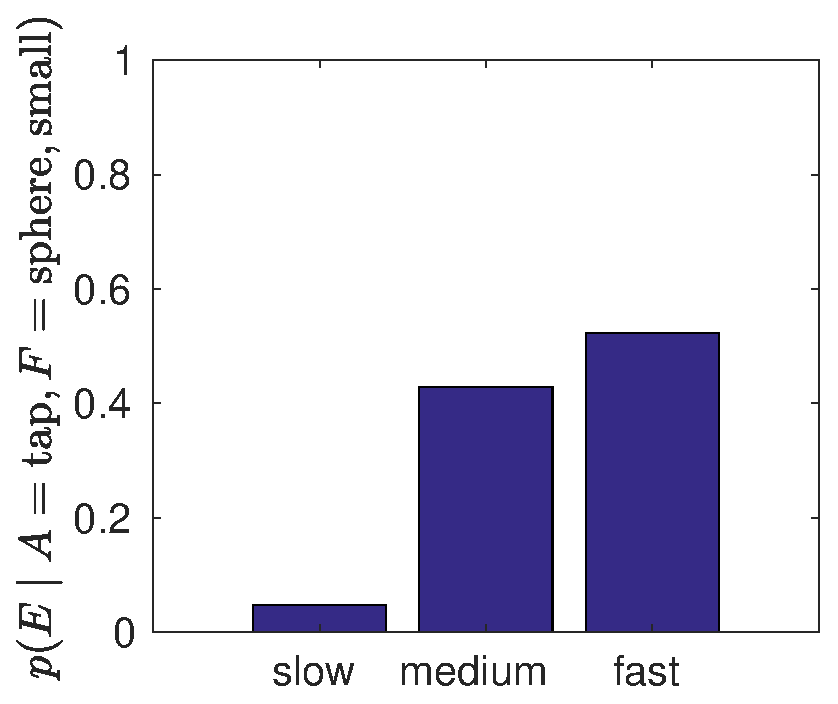
\includegraphics[width=0.45\linewidth]{effectpred_sphere.eps} \label{fig:effect_pred:sphere} } \quad
    %
    \subfloat[][Prediction of the movement effect on a big box.]
    { 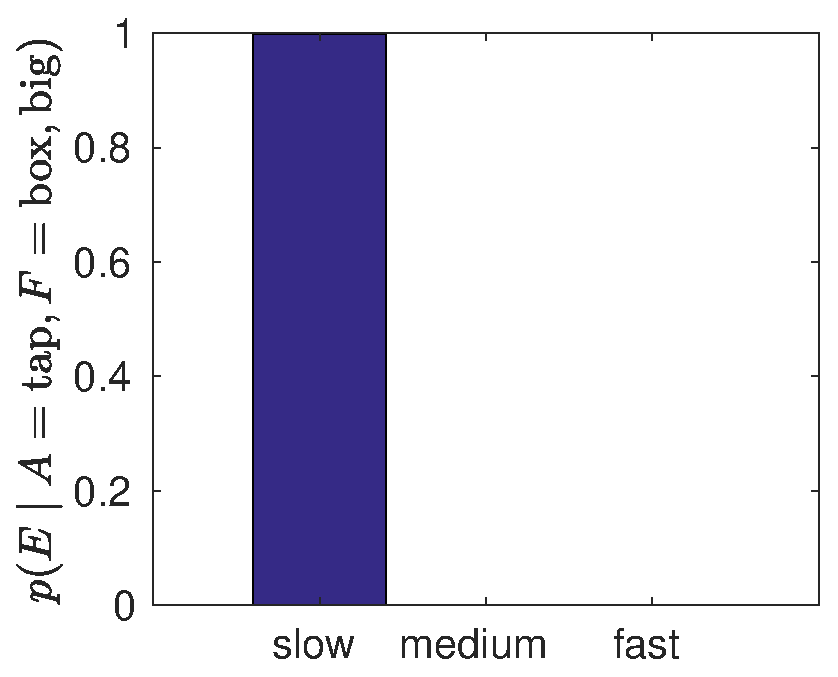
\includegraphics[width=0.45\linewidth]{effectpred_box.eps} \label{fig:effect_pred:box} }
    \caption{Object velocity predictions, given prior information~(from Gesture \acp{HMM}) that the human user performs a tapping action.}
    \label{fig:effect_pred}
\end{figure}

\subsection{Prediction of Words}

In this experiment, we compare the associated verbal description obtained by the \acl{BN} in the absence of an action prior, with the ones obtained in the presence of one. In particular, we compare the probability of word occurrence in these two situations:
\begin{enumerate}
\item when the robot prior knowledge~(evidence in the \ac{BN}) includes information about object features and effects only: \emph{Size=big, Shape=sphere, ObjVel=fast};

\item when the robot prior knowledge includes, in addition to the above, evidence about the action as observed from the Gestures \acp{HMM}, in particular \emph{Action=tap}.
\end{enumerate}

\begin{figure}
\centering
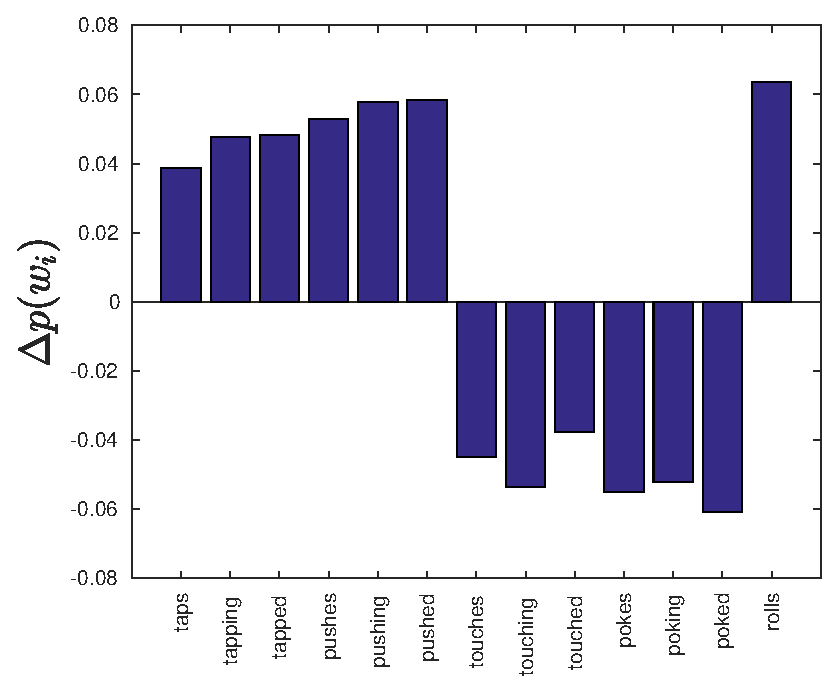
\includegraphics[width=0.9\columnwidth]{partialfig.eps}
\caption{Variation of word occurrence probabilities when we add the tap action evidence~(obtained from the Gesture \acp{HMM}) to the initial evidence about object features and effects.}
\label{fig:probdiff}
\end{figure}

Fig.~\ref{fig:probdiff} shows the variation in word occurrence probabilities between the two cases. We can interpret the difference in the predictions as follows:
\begin{itemize}
\item the probabilities of words related to tapping and pushing increase when a tapping action evidence from the Gestures \acp{HMM} is introduced; conversely, the probabilities of other action words~(touching and poking) decreases;

\item interestingly, the probability of the word \emph{rolling}~(which is an effect of an action onto an object) also increases when the tapping action evidence is entered. Even though the initial evidence of case~$1$ already included some effect information~(the velocity of the object), it is only now, when the robot perceives that the physical action was a tap, that the event rolling is associated.
\end{itemize}

%We compare the \ac{BN} predictive power in terms of word nodes, with and without the Action prior information provided by the Gesture \acp{HMM}. In other words, we compare~$p(W \mid A, E, F)$ with~$p(W \mid E, F)$.

%TODO work in progress, looking for a combination of E,F which makes the result significant
